\let\negmedspace\undefined
\let\negthickspace\undefined
\documentclass[journal]{IEEEtran}
\usepackage[a5paper, margin=10mm, onecolumn]{geometry}
%\usepackage{lmodern} % Ensure lmodern is loaded for pdflatex
\usepackage{tfrupee} % Include tfrupee package

\setlength{\headheight}{1cm} % Set the height of the header box
\setlength{\headsep}{0mm}     % Set the distance between the header box and the top of the text

\usepackage{gvv-book}
\usepackage{gvv}
\usepackage{cite}
\usepackage{amsmath,amssymb,amsfonts,amsthm}
\usepackage{algorithmic}
\usepackage{graphicx}
\usepackage{textcomp}
\usepackage{xcolor}
\usepackage{txfonts}
\usepackage{listings}
\usepackage{enumitem}
\usepackage{mathtools}
\usepackage{gensymb}
\usepackage{comment}
\usepackage[breaklinks=true]{hyperref}
\usepackage{tkz-euclide} 
\usepackage{listings}
% \usepackage{gvv}                                        
\def\inputGnumericTable{}                                 
\usepackage[latin1]{inputenc}                                
\usepackage{color}                                            
\usepackage{array}                                            
\usepackage{longtable}                                       
\usepackage{calc}                                             
\usepackage{multirow}                                         
\usepackage{hhline}                                           
\usepackage{ifthen}                                           
\usepackage{lscape}

\begin{document}

\bibliographystyle{IEEEtran}
\vspace{3cm}

\title{5.2.18}
\author{EE25BTECH11015 - Bhoomika V}
% \maketitle
% \newpage
% \bigskip
{\let\newpage\relax\maketitle}

\renewcommand{\thefigure}{\theenumi}
\renewcommand{\thetable}{\theenumi}
\setlength{\intextsep}{10pt} % Space between text and floats


\numberwithin{equation}{enumi}
\numberwithin{figure}{enumi}
\renewcommand{\thetable}{\theenumi}
\parindent 0px 
{Question :-} \\ 
Solve the following system of linear equation.\\ 
$8x + 5y = 9$\\ 
$3x + 2y = 4$\\ \\ 
\solution \\
We are solving the system:
\[
8x + 5y = 9, \quad 3x + 2y = 4
\]

Coefficient matrix and vector
\[
A = \begin{bmatrix} 8 & 5 \\ 3 & 2 \end{bmatrix}, \quad 
b = \begin{bmatrix} 9 \\ 4 \end{bmatrix}
\]

 Performing row operations (RREF)

\(R_1 \to \frac{R_1}{8}\)
\[
\begin{bmatrix} 8 & 5 \\ 3 & 2 \end{bmatrix} 
\;\overset{R_1 \to R_1/8}{\longrightarrow}\;
\begin{bmatrix} 1 & 5/8 \\ 3 & 2 \end{bmatrix}, \quad
b = \begin{bmatrix} 9 \\ 4 \end{bmatrix} 
\;\overset{R_1 \to R_1/8}{\longrightarrow}\;
\begin{bmatrix} 9/8 \\ 4 \end{bmatrix}
\]

Eliminate first column in \(R_2\): \(R_2 \to R_2 - 3R_1\)
\[
\begin{bmatrix} 1 & 5/8 \\ 3 & 2 \end{bmatrix} 
\;\overset{R_2 \to R_2 - 3R_1}{\longrightarrow}\;
\begin{bmatrix} 1 & 5/8 \\ 0 & 1/8 \end{bmatrix}, \quad
b = \begin{bmatrix} 9/8 \\ 4 \end{bmatrix} 
\;\overset{R_2 \to R_2 - 3R_1}{\longrightarrow}\;
\begin{bmatrix} 9/8 \\ 5/8 \end{bmatrix}
\]

\(R_2 \to 8R_2\)
\[
\begin{bmatrix} 1 & 5/8 \\ 0 & 1/8 \end{bmatrix} 
\;\overset{R_2 \to 8R_2}{\longrightarrow}\;
\begin{bmatrix} 1 & 5/8 \\ 0 & 1 \end{bmatrix}, \quad
b = \begin{bmatrix} 9/8 \\ 5/8 \end{bmatrix} 
\;\overset{R_2 \to 8R_2}{\longrightarrow}\;
\begin{bmatrix} 9/8 \\ 5 \end{bmatrix}
\]

Eliminate second column in \(R_1\): \(R_1 \to R_1 - (5/8)R_2\)
\[
\begin{bmatrix} 1 & 5/8 \\ 0 & 1 \end{bmatrix} 
\;\overset{R_1 \to R_1 - (5/8)R_2}{\longrightarrow}\;
\begin{bmatrix} 1 & 0 \\ 0 & 1 \end{bmatrix}, \quad
b = \begin{bmatrix} 9/8 \\ 5 \end{bmatrix} 
\;\overset{R_1 \to R_1 - (5/8)R_2}{\longrightarrow}\;
\begin{bmatrix} -1 \\ 5 \end{bmatrix}
\]

 Answer 
\[
x = -1, \quad y = 5
\]
\begin{figure}[H]
\begin{center}
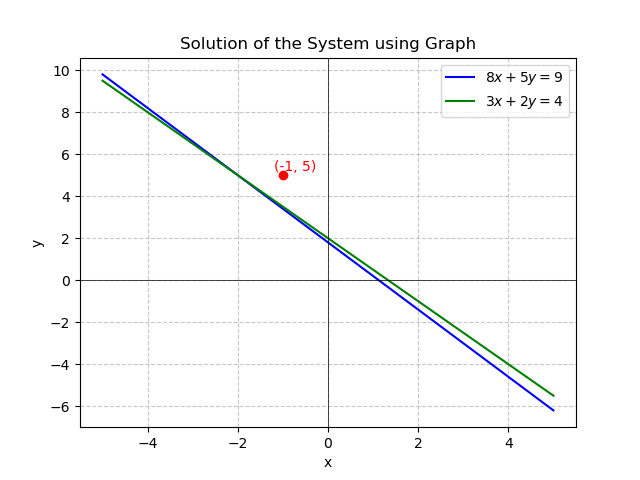
\includegraphics[width=0.6\columnwidth]{Figs/Fig1.png}
\end{center}
\caption{}
\label{fig:Fig.1}
\end{figure}


\end{document}
